\subsection{执行阶段性能剖析}\label{sec:execution}

执行阶段的任务，是把推理阶段给出的目标关节位置发送给机械臂的六个 STS-3215 舵机。
为了说明这条链路的真实约束，本节也把观测阶段中的舵机位置读取纳入分析。
写入目标位置和读取当前位置共用同一条半双工舵机总线、同一个 USB 串口设备以及同一套舵机协议，
区别只在于：写入是一次广播发送，读取得先发请求，再等待各个舵机依次回包。

\subsubsection{执行路径的软件关系}\label{sec:execution-software-stack}

图~\ref{fig:execution-callstack-software} 展示了执行阶段的关键软件关系：
主循环只负责发起动作发送或位置读取，真正处理关节值转换、符号方向和协议组包的是电机总线层，
最后再交给底层舵机库与串口设备。

从职责上看，读和写共用前半段软件链路：先把关节角度转换成舵机寄存器值，
再按舵机协议打包成串口字节。区别出现在总线方向上：
写入目标位置时，上层发出一条广播写帧即可返回；读取当前位置时，
上层必须等待六个舵机按编号顺序逐个返回状态帧。

\begin{figure}[htbp]
  \centering
  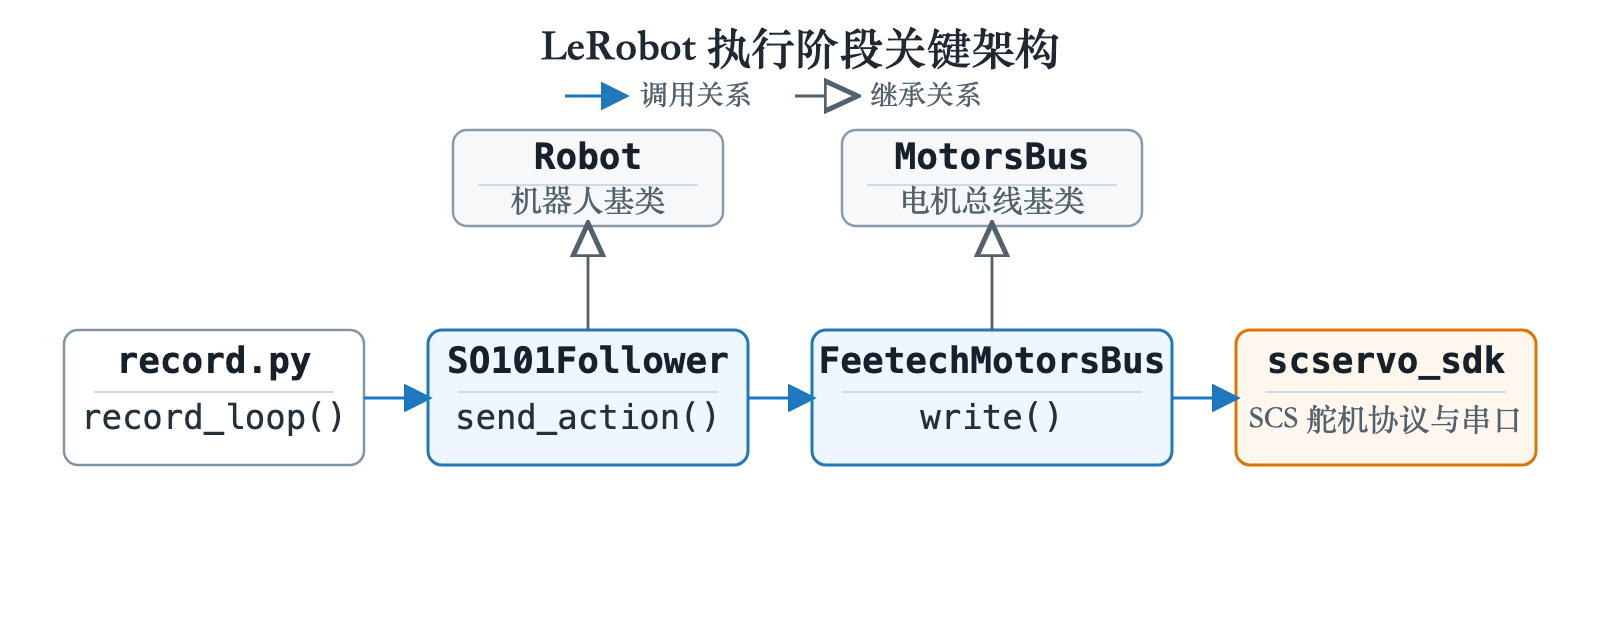
\includegraphics[width=\textwidth]{3_性能分析/image/execution_callstack_software.png}
  \caption{执行阶段关键软件关系}
  \label{fig:execution-callstack-software}
\end{figure}

\subsubsection{写入链路：从目标位置到串口}\label{sec:sync-write-chain}

图~\ref{fig:sync-write-chain} 展示了目标位置写入舵机的完整路径。
这条链路可以按职责理解为三步：电机总线层先把目标关节位置转换为舵机可识别的数值；
协议层把六个舵机的目标值合成一条广播写帧；串口层再把这段字节交给操作系统。

同步写初始化逻辑先设置目标位置寄存器地址 42 与数据长度 2 字节。
随后，每个舵机的目标位置被拆成低字节和高字节，并放入组包缓冲区；
底层库再将 6 个舵机的数据拼成负载，追加协议头与校验字节，
构造出表~\ref{tab:sync-write-packet} 所示的 26 字节同步写广播帧。

\begin{table}[htbp]
  \centering
  \caption{同步写广播帧结构}
  \label{tab:sync-write-packet}
  \small
  \renewcommand{\arraystretch}{1.12}
  \begin{tabularx}{\textwidth}{@{}p{2.4cm}p{3.1cm}p{2.8cm}X@{}}
    \toprule
    字段 & 字节 & 长度 & 含义 \\
    \midrule
    帧头 & \texttt{FF FF} & 2 字节 & 舵机协议同步头 \\
    目标编号 & \texttt{FE} & 1 字节 & 广播地址，所有舵机接收该写指令 \\
    长度 & \texttt{16} & 1 字节 & 后续字段长度为 22 字节 \\
    指令 & \texttt{83} & 1 字节 & 同步写指令 \\
    起始地址 & \texttt{2A} & 1 字节 & 目标位置寄存器地址，即十进制 42 \\
    数据长度 & \texttt{02} & 1 字节 & 每个舵机写入 2 字节目标位置 \\
    舵机数据 & 编号、低字节、高字节 × 6 & 18 字节 & 每个舵机占 1 字节编号和 2 字节位置值 \\
    校验 & \texttt{CS} & 1 字节 & 协议校验字节 \\
    \bottomrule
  \end{tabularx}
\end{table}

由于目标编号是广播地址，舵机收到目标位置后不会返回状态包。
因此，上层只需要把广播帧写入串口；一旦操作系统接受这段字节，
写入调用就可以返回，后续不再进入接收阶段。

写链路的核心特性是``发完即返回''——广播帧不要求舵机回包，上层耗时约
1--3 ms。这里的主要开销是 USB 串口和舵机总线的物理传输时间，
而不是上层软件封装本身。

\begin{figure}[htbp]
  \centering
  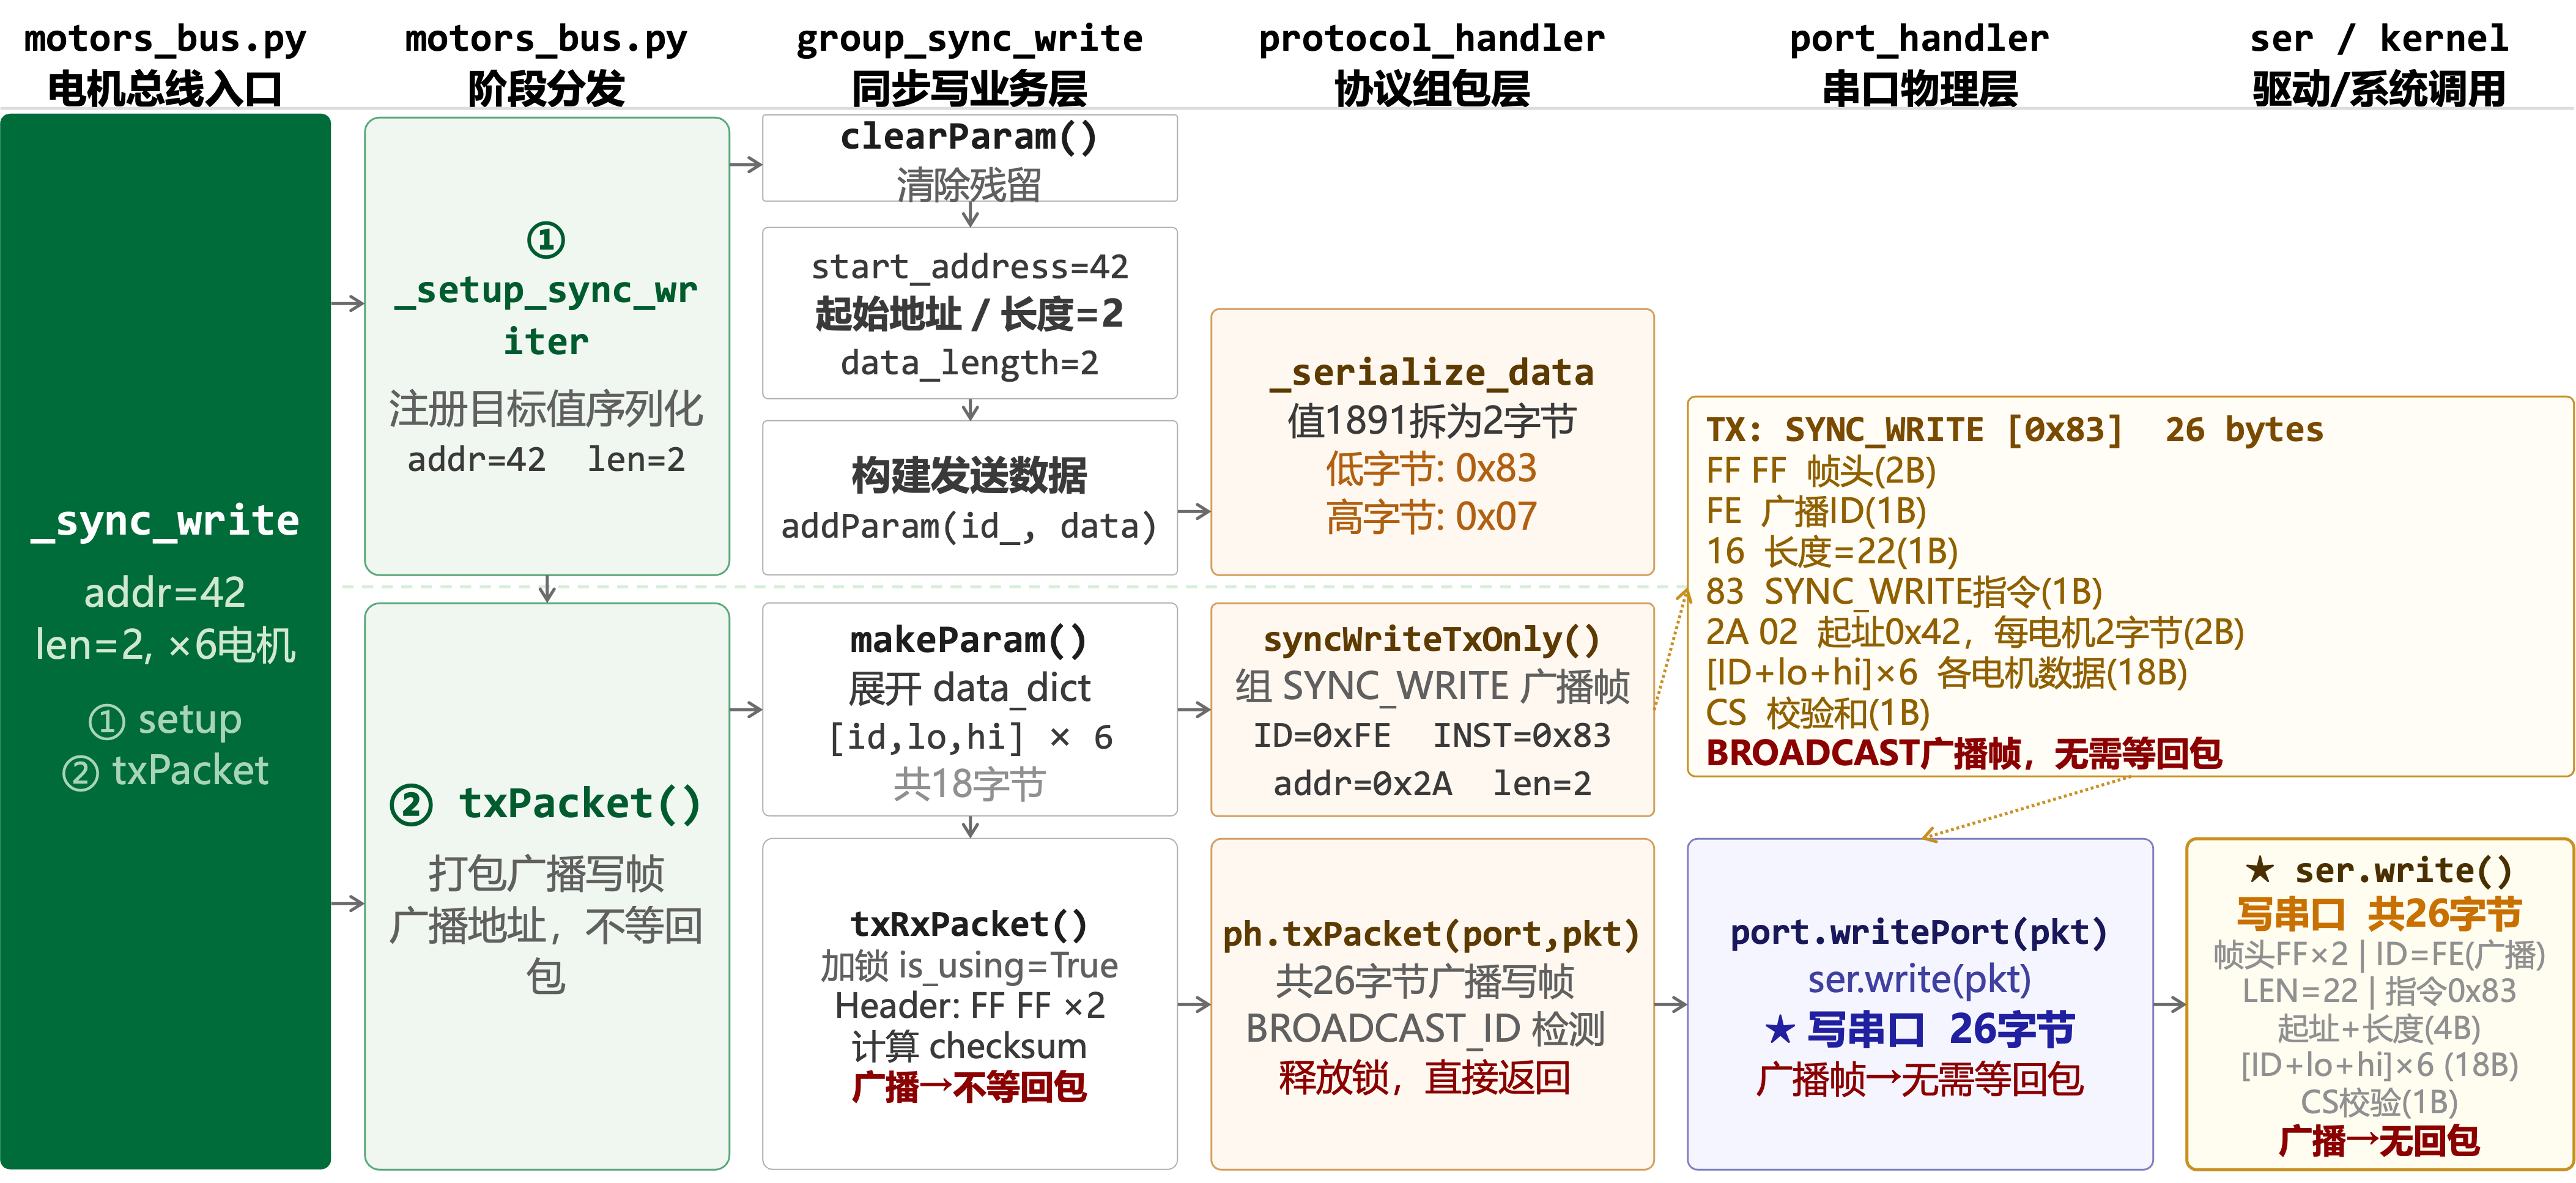
\includegraphics[width=\textwidth]{3_性能分析/image/sync_write_chain.png}
  \caption{同步写入链路}
  \label{fig:sync-write-chain}
\end{figure}

继续向内核下钻时，需要区分``串口抽象''和``真实硬件通道''。
对应用程序而言，\texttt{/dev/ttyACM0} 像一个普通串口文件，写入动作就是向这个文件发送一段舵机协议字节。
但树莓派 5 上这一路并不是片上原生串口，而是一个 USB 串口设备：
操作系统把它包装成串口，底层实际仍通过 USB 控制器完成传输。

进入内核后，通用文件层先完成写入检查，再把数据交给终端字符设备层。
在当前原始串口模式下，终端层不会解释或修改舵机协议，只是把字节继续交给 USB 串口驱动。
随后，USB 串口驱动把这段舵机协议字节封装成 USB 传输请求，
提交给 USB 核心和主机控制器。到这一步，系统调用即可返回；
后续由硬件控制器继续把数据包发到总线上。因此，系统调用返回只表示内核已经接收并提交了这批字节，
并不等价于六个舵机已经完成动作执行。

\begin{figure}[htbp]
  \centering
  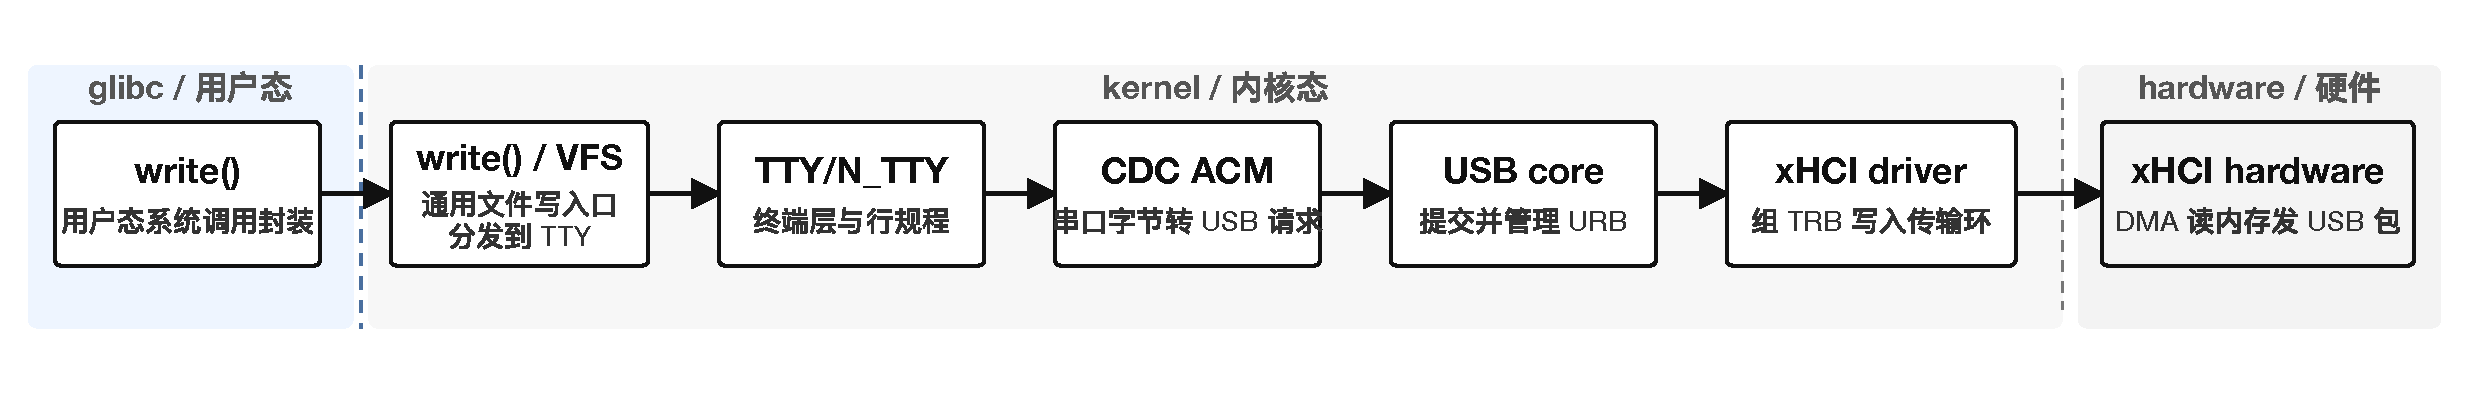
\includegraphics[width=0.95\textwidth]{3_性能分析/image/write_kernel_chain.pdf}
  \caption{串口写入进入内核后的主链路}
  \label{fig:write-kernel-chain}
\end{figure}

\subsubsection{读取链路：从请求帧到逐电机回包}\label{sec:sync-read-chain}

图~\ref{fig:sync-read-chain} 展示了读取舵机当前位置的链路。
它与写链路共用前半段的电机总线层和协议组包层，
但进入串口之后就不再是单向发送，而是先发出读请求，
再等待各个舵机依次返回当前位置。

读链路中最容易混淆的是总线上实际出现的两类协议包。表~\ref{tab:sync-read-packet}
将同步读请求帧和单个舵机返回的状态帧拆开列出；请求帧只发送一次，
随后 6 个舵机按编号顺序依次返回状态帧。

\begin{table}[htbp]
  \centering
  \caption{同步读请求帧与单电机状态回包}
  \label{tab:sync-read-packet}
  \small
  \renewcommand{\arraystretch}{1.12}
  \begin{tabularx}{\textwidth}{@{}p{2.2cm}p{2.3cm}p{2.6cm}X@{}}
    \toprule
    包类型 & 字段 & 字节 & 含义 \\
    \midrule
    请求帧 & 帧头 & \texttt{FF FF} & 舵机协议同步头 \\
    & 目标编号 & \texttt{FE} & 广播地址，表示一次请求覆盖多个舵机 \\
    & 长度 & \texttt{0A} & 后续字段长度，包括指令、参数和校验 \\
    & 指令 & \texttt{82} & 同步读指令 \\
    & 起始地址 & \texttt{38} & 当前位置寄存器地址，即十进制 56 \\
    & 读取长度 & \texttt{02} & 每个舵机读取 2 字节位置值 \\
    & 编号列表 & \texttt{01 ... 06} & 依次读取 6 个舵机 \\
    & 校验 & \texttt{CS} & 协议校验字节 \\
    \midrule
    状态回包 & 帧头 & \texttt{FF FF} & 舵机状态帧同步头 \\
    & 电机编号 & 编号值 & 当前返回数据的舵机编号 \\
    & 长度 & \texttt{04} & 错误码、2 字节数据和校验 \\
    & 错误码 & \texttt{00} & 正常回包 \\
    & 位置数据 & 低字节、高字节 & 低字节在前，高字节在后 \\
    & 校验 & \texttt{CS} & 协议校验字节 \\
    \bottomrule
  \end{tabularx}
\end{table}

因此，读取链路可以概括为三步：先按表~\ref{tab:sync-read-packet} 的前半部分构造读请求，
并通过同一条串口写路径发到总线上；随后，底层库按舵机编号逐个等待状态帧；
最后，从每个状态帧中取出低字节和高字节，合成为 16 位当前位置。
由于总线为半双工结构，等待回包期间不能同时发送其他指令。

读链路耗时约 1.2 ms，主要来源于 6 次串行回包等待。半双工总线在等待回包期间
不能发送任何其他指令，这是写链路无法与读链路并行化的物理根因。

\begin{figure}[htbp]
  \centering
  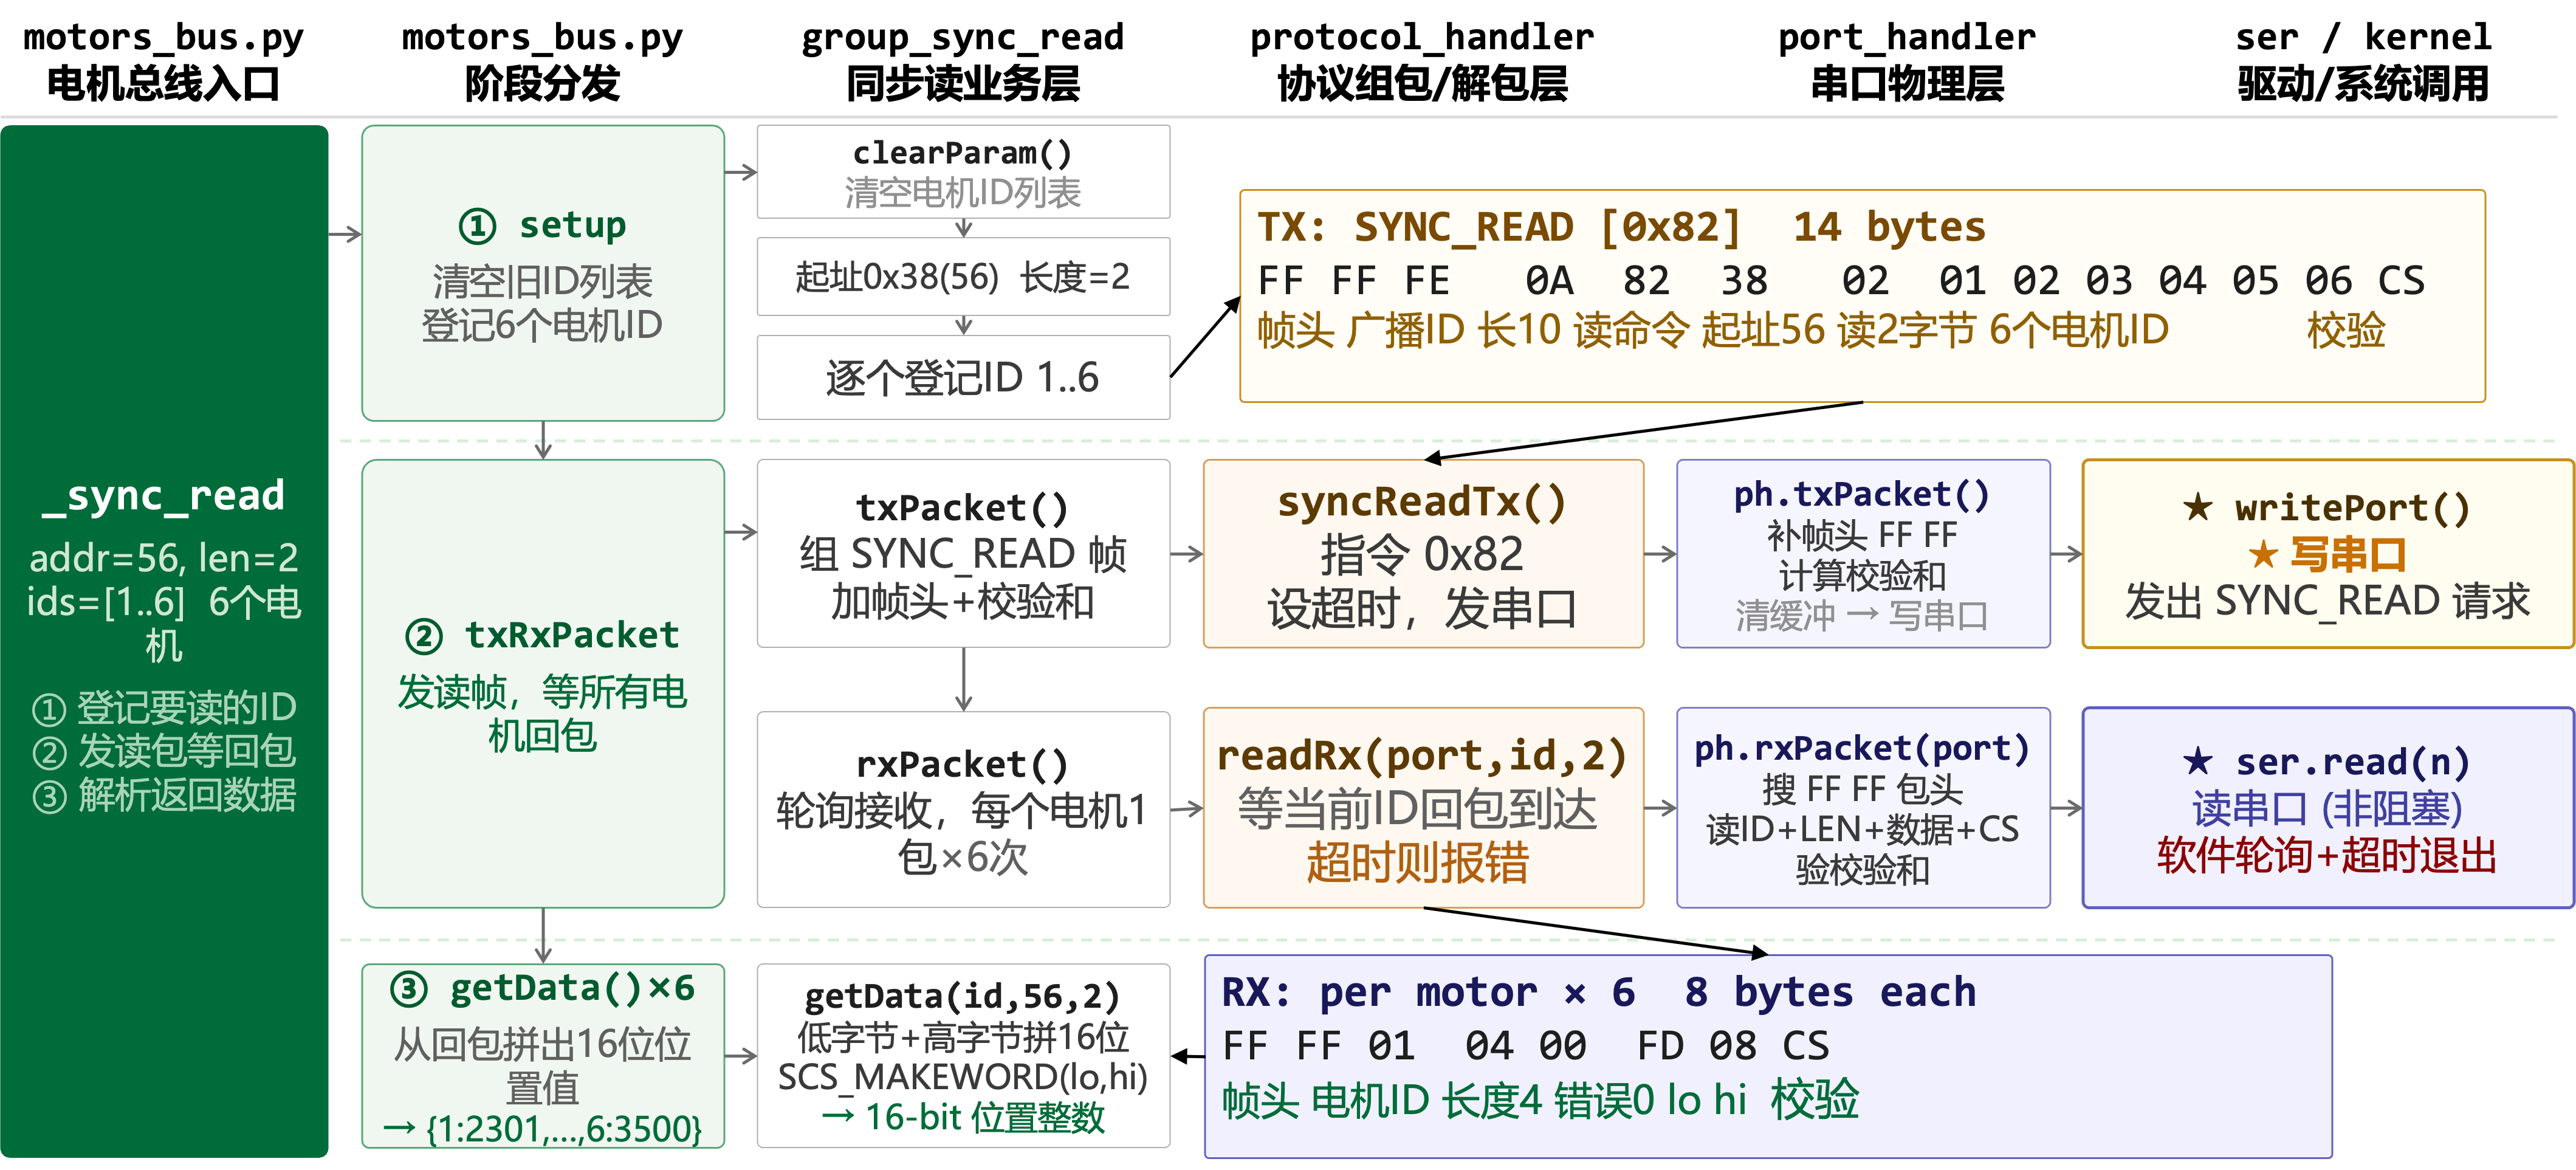
\includegraphics[width=\textwidth]{3_性能分析/image/sync_read_chain.png}
  \caption{同步读取链路：请求组包、请求写出、逐电机回包与数据解析}
  \label{fig:sync-read-chain}
\end{figure}

\textbf{关键性能结论}\label{sec:execution-conclusion}：
综合读取和写入两条路径可以看出，执行阶段的主要耗时并不来自系统调用本身。
实际测得的串口写入系统调用只有约 38 $\mu$s，读取系统调用也处于类似量级；
而完整读取当前位置约 1.2 ms，写入目标位置约 1--3 ms。
这说明瓶颈主要由 1 Mbps 波特率下的舵机总线传输决定，而不是上层语言、
舵机库封装或内核调用路径决定。

从协议字节数也能得到同样结论：同步读请求帧约 14--15 字节，
同步写广播帧约 26 字节，其中六个舵机的数据项占主要部分。
这些字节必须在半双工总线上串行传输，因此同一时刻总线只能容纳一个方向的通信。
如果把读写简单地异步并发，反而可能造成总线竞争或指令帧损坏。
同时，动作发送前的安全限幅依赖实时读取到的当前位置；
若把舵机读写拆成不受约束的异步流程，会破坏这一控制不变量。
因此，舵机读写不适合作为本文主要异步优化方向（详见 \S\ref{sec:async-feasibility}）。
